\documentclass[watermark]{pbpreprint}
\usepackage{listings}
\usepackage{bold-extra}
\usepackage{wasysym}
\usepackage{tikz}
\usetikzlibrary{backgrounds}
\usetikzlibrary{calc}


\newsubfloat{table}

\DeclareFontEncoding{LS1}{}{}
\DeclareFontSubstitution{LS1}{stix}{m}{n}
\DeclareSymbolFont{arrows1}{LS1}{stixsf}{m}{n}
\DeclareMathSymbol{\nicearrow}{\mathrel}{arrows1}{"B1}

\newcommand*\keystroke[1]{%
  \begin{tikzpicture}[baseline=(key.base), very thin, line cap=round, black, rounded corners=0pt]%
    \node [draw, fill=white, fill opacity=1, rectangle, rounded corners=2pt, inner sep=1pt, minimum width=1.2em, font=\scriptsize\sffamily] (key) {#1\strut};

    \begin{scope}[on background layer]
      \draw [rounded corners=1pt, fill=white] ($ (key.north west) + (-2pt, 2pt) $) rectangle ($ (key.south east) + (2pt, -2pt) $);

      \fill [gray!60] ($ (key.south west) + (2pt, 0.1pt) $) -- ($ (key.south west) + (-1pt, -2pt) $)
                  -- ($ (key.south east) + (1pt, -2pt) $)  -- ($ (key.south east) + (-2pt, 0.1pt) $) -- cycle;

      \fill [gray!60] ($ (key.south east) + (-0.1pt, 2pt) $) -- ($ (key.south east) + (2pt, -1pt) $)
                  -- ($ (key.north east) + (2pt, 1pt) $)    -- ($ (key.north east) + (-0.1pt, -2pt) $) -- cycle;
    \end{scope}

    \draw ($ (key.north west) + (0.1pt, -2pt) $) -- ($ (key.north west) + (-2pt, 1pt) $);
    \draw ($ (key.north west) + (2pt, -0.1pt) $) -- ($ (key.north west) + (-1pt, 2pt) $);

    \draw ($ (key.north east) + (-0.1pt, -2pt) $) -- ($ (key.north east) + (2pt, 1pt) $);
    \draw ($ (key.north east) + (-2pt, -0.1pt) $) -- ($ (key.north east) + (1pt, 2pt) $);

    \draw ($ (key.south west) + (0.1pt, 2pt) $) -- ($ (key.south west) + (-2pt, -1pt) $);
    \draw ($ (key.south west) + (2pt, 0.1pt) $) -- ($ (key.south west) + (-1pt, -2pt) $);

    \draw ($ (key.south east) + (-0.1pt, 2pt) $) -- ($ (key.south east) + (2pt, -1pt) $);
    \draw ($ (key.south east) + (-2pt, 0.1pt) $) -- ($ (key.south east) + (1pt, -2pt) $);
  \end{tikzpicture}%
}


\begin{document}
\title{Storing and transferring files}
\newcommand{\subtitle}{Big Data in Life Science}
\renewcommand{\maketitlehookb}{\centering\textsc{\subtitle}}
\author{Jonathan Alvarsson}
\maketitle
\begin{KeepFromToc}
   \tableofcontents
\end{KeepFromToc}

\definecolor{light-gray}{gray}{0.96}
\lstset{basicstyle=\ttfamily\small, frame = single, backgroundcolor = \color{light-gray}}

\section{Introduction}
In this lab we will try out different approaches to transferring and storing
files. Our files will not quite qualify as being big data instead we will focus
on getting a chance to test different tools. Much of what we will do will be to
copy files from one location to another. Although you are free to use whatever
locations you want I will suggest that you work inside your assigned Kubernetes
pods (also known as Jupyter notebooks) on the cluster by accessing a terminal
there and then copy things to your Uppmax account. This is the best way because
your pods are not configured to accept any connections from the outside whereas
the Uppmax systems are.

\section{Downloading from the Zink database using \texttt{wget}}
\marginpar{\textit{Follow along and run the commands on your own. These
instructions will assume that you run things and won't show any output from the
commands so in order to understand what is going on you need to run all the
commands and look at the output\ldots}~\smiley{}}
Zink is ``a freely available database of commercially-available compounds for
virtual screening'', we will be using the 2012 version and download some
datasets from it. On \url{http://zinc12.docking.org/subsets/lead-like} there
are a lot of datasets listed if you click on the \texttt{Downloads} tab. The
molecules can be downloaded in different formats. Let's start by grabbing all
of them in the SMILES format using \texttt{wget}:
\sidepar{\vspace{12.5pt}\textbf{\texttt{wget}}}
\begin{lstlisting}[language=bash]
$ wget http://zinc12.docking.org/db/bysubset/1/1_p0.smi.gz
\end{lstlisting}
We have now downloaded a gzipped text file. We can have a look at it using
\texttt{zless}:
\sidepar{\vspace{12.5pt}\textbf{\texttt{zless}}}
\begin{lstlisting}[language=bash]
$ zless 1_p0.smi.g
\end{lstlisting}
As you can see the file contains two columns. The first column is the SMILES
string and the second column is an identifier. The simplified molecular-input
line-entry system (SMILES) is a way to write down a molecular structure as a
string. We can also unpack it using \texttt{gunzip}:%
\sidepar{\vspace{12.5pt}\textbf{\texttt{gunzip}}}%
\begin{lstlisting}[language=bash]
$ gunzip 1_p0.smi.gz
\end{lstlisting}
Now by default this will remove the original file and leave only the unpacked
file. With \texttt{gzip} we can compress it again:
\sidepar{\vspace{12.5pt}\textbf{\texttt{gzip}}}
\begin{lstlisting}[language=bash]
$ gzip 1_p0.smi
\end{lstlisting}
Now if we want to unpack it and still keep the packaged version we can do this like:
\begin{lstlisting}[language=bash]
$ gunzip -k 1_p0.smi.gz
\end{lstlisting}
the \texttt{-k} flag (as in ``keep'') works for \texttt{gzip} as well. 

\vspace{1\baselineskip}
Now, let's take this opportunity to see how big the files was compressed and
unpacked, run: 
\begin{lstlisting}[language=bash]
$ ls -lh
\end{lstlisting}
\texttt{ls} is the command to list files, \texttt{-l} means that you want the
long version of the output that show size and \texttt{-h} means that you want
the file sizes in human readable numbers. Without the \texttt{-h} you will get
the file size in bytes. When giving many flags to a command like this you can
just squish them together and write \texttt{-lh} instead of \texttt{-l -h}.

\section{Transfer file using \texttt{scp}}
\marginpar{\textit{Although \texttt{scp} is considered ``outdated, inflexible and not
readily fixed'', it can be good to have seen it in action in case you stumble
upon it being used somewhere.}} We will use \texttt{scp} to copy from the terminal
in Jupyter Lab to our account on Uppmax. I will be using my username
\texttt{jonathan} and \texttt{rackham} in the examples. You need to replace
this as appropiate. Let's transfer the file \texttt{1\_p0.0.sdf.gz} that we
downloaded from the Zink webserver:
\sidepar{\vspace{14pt}\textbf{\texttt{scp}}}
\begin{lstlisting}[language=bash,escapechar={|}]
$ scp 1_p0.0.sdf.gz jonathan@rackham.uppmax.uu.se:|$\sim$|
\end{lstlisting}
\texttt{scp} is the name of the command, next follows the file that we want to
copy, after that we need to specify whereto we want to copy the file. The way
we do this is to write our username followed by the @ symbol and then address
fro the computer we want to copy the file to. We then write a : symbol and then
where on this computer the file should be placed. The symbol $\sim$ in this
case means put it in the home directory of the user, in this case the home
directory of the user \texttt{jonathan}.

\section{Transfer file using SFTP}
\texttt{sftp} is in fact slower than \texttt{scp} when it comes to copying
files. It is a bit of an unfair comparison though because \texttt{sftp} allows
for browsing files, removing remote files, and resuming interrupted transfers
in addition to copying them.

Now, let's create a directory in our home remote home folder and copy our
file into it using \texttt{sftp}. 
\sidepar{\vspace{14pt}\textbf{\texttt{sftp}}}
\begin{lstlisting}[language=bash,escapechar={|}]
$ sftp jonathan@rackham.uppmax.uu.se
\end{lstlisting}
First we establish a connection to the remote computer. We can now list files
on the remote computer much like we would using standard bash:
\marginpar{\textit{Notice that when we are working in the established
\texttt{sftp} connection the prompt has changed to reflect this.}}
\begin{lstlisting}[language=bash,escapechar={|}]
sftp> ls
\end{lstlisting}
Now we create a folder \texttt{test\_folder}:
\begin{lstlisting}[language=bash,escapechar={|}]
sftp> mkdir test_folder
\end{lstlisting}
change remote working directory to it:
\begin{lstlisting}[language=bash,escapechar={|}]
sftp> mkdir test_folder
\end{lstlisting}
and upload (put) our file there:
\begin{lstlisting}[language=bash,escapechar={|}]
sftp> put 1_p0.0.sdf
\end{lstlisting}
If you want forget the name of the file you want to upload you can list your local files with:
\begin{lstlisting}[language=bash,escapechar={|}]
sftp> lls
\end{lstlisting}
and if you forget what your current remote working directory is you can show it
by:
\begin{lstlisting}[language=bash,escapechar={|}]
sftp> pwd
\end{lstlisting}

\vspace{1\baselineskip}
There are more commands available in \texttt{sftp} but we will stop here. When
you are done you can do either \keystroke{Ctrl} + \keystroke{D} or write:
\vspace{3pt}
\begin{lstlisting}[language=bash,escapechar={|}]
sftp> bye
\end{lstlisting}

\section{Synchronize file with \texttt{rsync}}
\texttt{rsync} was born out of the frustration of waiting for complete files to
be transferred over slow connections when in fact only parts of the files had
been changed and thus only the changed parts really ought to need to be
transferred. \texttt{rsync} does this by comparing the files on both systems
and then only transferring the changes. It can also be used on entire file
hierarchies. 

Let's start out by copying our unpacked file \texttt{1\_p0.smi} to Uppmax using
\texttt{rsync}:
\sidepar{\vspace{14pt}\textbf{\texttt{rsync}}}
\begin{lstlisting}[language=bash,escapechar={|},basicstyle=\ttfamily\footnotesize]
$ rsync -z -P 1_p0.smi jonathan@rackham.uppmax.uu.se:|$\sim$|/1_p0.smi
\end{lstlisting}
By now you probably recognize the general form of these commands. We want to
copy \texttt{1\_p0.smi} to \texttt{jonathan@rackham.uppmax.uu.se:$\sim$/1\_p0.smi}
using \texttt{rsync}. \marginpar{\textit{Waiting for something that gives no
signs of progress at all can be very frustrating. So it is often worth
activating progress monitors in software.}} I added two flags \texttt{-z} which
tells \texttt{rsync} to use compression during transfer, if you want to you can
try without it, it makes quite a big difference to transfer speed, and
\texttt{-P} which tells \texttt{rsync} to write some information about how much
of the file has been transferred and how much time is left to the terminal,
\texttt{-P} also tells \texttt{rsync} not to remove partially transferred files
if connection is broken. This means that \texttt{rsync} can continue where it
failed thus making subsequent transfer of the rest of that file much faster. 

Now let's try to change something in our file and then run \texttt{rsync}
again. The file \texttt{1\_p0.smi} contains SMILES and id on each row so the
easiest way to edit the file without ``breaking'' it is to remove a row or two.
Open the file in your favourite text editor and remove a couple of rows.

If we now rerun the \texttt{rsync} command the transfer should be almost
instantaneous:
\sidepar{\vspace{14pt}\textbf{\texttt{rsync}}}
\begin{lstlisting}[language=bash,escapechar={|},basicstyle=\ttfamily\footnotesize]
$ rsync -z -P 1_p0.smi jonathan@rackham.uppmax.uu.se:|$\sim$|/1_p0.smi
\end{lstlisting}

\section{More about \texttt{zip}}
We will now look a bit further at the working with zip files. First let's
download a zip file that we can try things on:
\sidepar{\vspace{14pt}\textbf{\texttt{wget}}}%
\marginpar{\vspace{-2\baselineskip}\textit{I am using the
\mbox{\textcolor{red}{$\nicearrow$}} symbol where I am forced to break lines of
code because on paper the horizontal space is limited.}}
\begin{lstlisting}[language=bash,escapechar={|},basicstyle=\ttfamily\footnotesize,breaklines=true,
           postbreak=\mbox{\textcolor{red}{$\nicearrow$}\space}]
$ wget https://pubs.acs.org/doi/suppl/10.1021/ci500361u/suppl_file/ci500361u_si_002.zip
\end{lstlisting}
So, the downloaded file is about 13\,MB and we can use the \texttt{unzip} command to list the content of it:
\sidepar{\vspace{14pt}\textbf{\texttt{unzip}}}%
\begin{lstlisting}[language=bash,escapechar={|},basicstyle=\ttfamily\footnotesize]
$ unzip -l ci500361u_si_002.zip
\end{lstlisting}
The flag \texttt{-l} in this case means list the content of the zip archive. As you can
see there are quite a few files in this zip archive. Let's say that we are
interested in just the predictions, they are in \texttt{.csv} files in the
\texttt{Predictions} directory so to unpack only them we can do:
\sidepar{\vspace{14pt}\textbf{\texttt{unzip}}}%
\begin{lstlisting}[language=bash,escapechar={|},basicstyle=\ttfamily\footnotesize]
$ unzip ci500361u_si_002.zip Predictions/*
\end{lstlisting}
Next let's also create a zip file using this command line tool. We can pack
those prediction \texttt{.csv} files into a new \texttt{.zip} file like:
\sidepar{\vspace{14pt}\textbf{\texttt{zip}}}%
\begin{lstlisting}[language=bash,escapechar={|},basicstyle=\ttfamily\footnotesize]
$ zip -v predictions.zip Predictions/* 
\end{lstlisting}
the \texttt{-v} flag means verbose, it gives some extra output which probably
is not that interesting in general but I thought it could be interesting
for you to look at this time. 

\section{The \texttt{tar.gz} approach -- package multiple files into one \texttt{.gz} file}
As already mentioned \texttt{gzip} is a program for compressing a file, but
what if we want to compress more than one file? There is however another
program available for collecting many files into one, it is called
\texttt{tar}. Once we have created a \texttt{tar} archive we can compress it
using \texttt{gzip}, this is an example of a common design principle in the
Unix world where each program focuses on solving one problem well and can be
used as building peaces to accomplish something bigger. However, in fact the
\texttt{tar} command has a flag (\texttt{-z}) for compressing a \texttt{.tar}
file using \texttt{gzip} while creating it. So, let's use our predictions
\texttt{.csv} files again:
\sidepar{\vspace{14pt}\textbf{\texttt{tar}}}%
\begin{lstlisting}[language=bash,escapechar={|},basicstyle=\ttfamily\footnotesize]
$ tar -cvzf predictions.tar.gz Predictions/ 
\end{lstlisting}
now, this is where things get complicated, \texttt{-cvzf}, that's quite a few
letters. Let's take them one at a time: \texttt{c} means create a new archive,
\texttt{v} means verbosely show the progress \texttt{z} means compress it using
\texttt{gzip} and \texttt{f} means directly after this follows the name that I
want the new archive file to have

Now, let's list the files in this archive:
\sidepar{\vspace{14pt}\textbf{\texttt{tar}}}%
\begin{lstlisting}[language=bash,escapechar={|},basicstyle=\ttfamily\footnotesize]
$ tar -tvf predictions.tar.gz 
\end{lstlisting}
\texttt{v} and \texttt{f} we are familiar with and
\texttt{-t}\marginpar{\vspace{-4\baselineskip}\textit{Notice that the short hand
version of list is \texttt{-t}, I guess \texttt{-l} was already taken\ldots\
Most of the commands also have long version, for example \texttt{-t} can be
written as \texttt{--list} but I was not sure how much that would help you so I
didn't include all the long versions}} means list the file content. To unpack
the archive we write:
\sidepar{\vspace{14pt}\textbf{\texttt{tar}}}%
\begin{lstlisting}[language=bash,escapechar={|},basicstyle=\ttfamily\footnotesize]
$ tar -xvf predictions.tar.gz 
\end{lstlisting}
again, \texttt{v} and \texttt{f} are familiar and to extract the archive we use
\texttt{-x}. Do you find the syntax of the \texttt{tar} command to be a bit
complicated? Well, if so you are not alone (see for example
Figure~\ref{xkcdtar}).

\begin{figure}[bht]
    \centering
    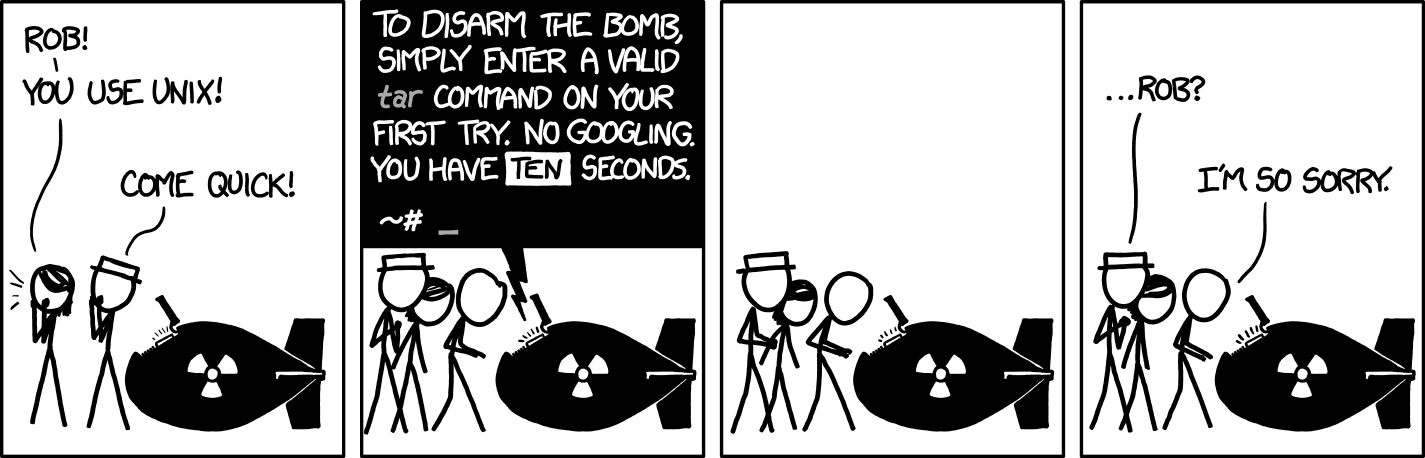
\includegraphics[width=0.8\textwidth]{Figures/xkcd_tar.png}\\
    \url{https://xkcd.com/1168/}
    \caption{The hoover text for this one is: \textit{``I don't know what's worse--the
    fact that after 15 years of using tar I still can't keep the flags
    straight, or that after 15 years of technological advancement I'm still
    mucking with tar flags that were 15 years old when I started.''}, and that
    sums it up pretty well. Sometimes old tools are old.\label{xkcdtar}}
\end{figure}

\section{Summary}
So, to sum up. We have used four different programs to transfer a file between
two computers. \texttt{wget} for downloading from the web,  \texttt{scp} for
copying files between computers, \texttt{sftp} for not just copying files but
for working with files and \texttt{rsync} for not just copying files but also
synchronising entire file hierarchies. In general you will use \texttt{wget}
for downloading files from the web, \texttt{rsync} for copying files between
computers, for few small files \texttt{scp} works fine and is perhaps a bit
easier to use but it mainly depends on what you are used to. When you need to
do more than just copying files you can use \texttt{sftp} but for just copying
\texttt{rsync} is probably faster.

We have also looked at two programs for compressing files. \texttt{zip} being
probably the most common format for compressing files in the Windows and Mac
world and \texttt{gzip} which is traditionally mainly used in the Unix / Linux
world. One benefit of \texttt{gzip} is the z tools that can operate on
\texttt{gzip}ed files and one benefit of the \texttt{zip} format is that files
can accessed randomly, \textit{i.e.}, you can unpack only the specific file you
are interested in from an archive. We also looked a bit at the \texttt{tar}
program for combining multiple files into one file and compressing that with
\texttt{gzip}.

\end{document}
